\documentclass[conference,10pt]{IEEEtran}
\usepackage{amsmath,amssymb,booktabs,graphicx,microtype,url}
\usepackage[caption=false,font=footnotesize]{subfig}
\hfuzz=1pt
\title{Minority-to-Majority Incremental Class Learning on Two Imbalanced Data Sets}
\author{\IEEEauthorblockN{PLACEHOLDER AUTHOR}
\IEEEauthorblockA{Student number: PLACEHOLDER STUDENT NUMBER\\
PLACEHOLDER INSTITUTION\\Module: PLACEHOLDER MODULE\\
Repository: \url{PLACEHOLDER HTTPS REPOSITORY URL}}}

\begin{document}
\nocite{bengio2009curriculum,buscema2010steel,he2009learning,koklu2020multiclass,parisi2019continual,sokolova2009systematic,yoon2018den}
\maketitle

\begin{abstract}
The investigation evaluated minority-to-majority class presentation on the Dry Bean and Steel Plates Faults datasets. Five outer folds and fold-specific training and validation splits protected test observations during model selection. Fixed incremental learning exceeded its update-budget control by 0.0007 and 0.0047 in test Macro-F1 on Dry Bean and Steel Plates, respectively. Dynamic incremental learning exceeded dynamic all-classes by 0.0011 and 0.0037. Every primary 95\% confidence interval included zero, and no Holm-adjusted test established a reliable difference. Fixed incremental learning achieved the highest overall and minority-class means. Dynamic methods used approximately two to five hidden units on average but required more gradient updates and achieved lower absolute Macro-F1 than the fixed methods. Five overlapping training partitions limited inference.
\end{abstract}
\begin{IEEEkeywords}class imbalance, curriculum learning, incremental learning, dynamic neural networks\end{IEEEkeywords}

\section{Introduction}
Class imbalance complicates multiclass evaluation. Frequent classes dominate aggregate accuracy under severe imbalance~\cite{he2009learning}. Minority-to-majority presentation offers a possible way to change learning priorities. The investigation evaluated the resulting classification performance and the cost of validation-triggered network growth.

The first research question concerned the predictive effect of minority-first presentation. The second research question concerned the performance--size trade-off produced by dynamic growth. Dry Bean~\cite{koklu2020multiclass} and Steel Plates Faults~\cite{buscema2010steel} supplied two naturally imbalanced problems from the University of California Irvine Machine Learning Repository.\footnote{University of California Irvine Machine Learning Repository: \url{https://archive.ics.uci.edu/}}

The fixed-capacity comparison controlled the number of gradient updates. The dynamic comparison controlled the complete capacity-growth policy. Update-budget matching did not equalise parameter count, examples processed, matrix-operation cost, or wall-clock time. The two controls therefore addressed different potential explanations for observed performance differences.

\section{Background}
Class-balanced evaluation, ordered presentation, and network expansion motivate the experimental comparisons.

\subsection{Imbalance and Evaluation}
Previous research showed a coincidence between high accuracy and weak rare-class performance~\cite{he2009learning}. A class-specific F1 score is the harmonic mean of precision and recall. Macro-averaged F1 score averages the class-specific F1 scores and assigns equal weight to every class~\cite{sokolova2009systematic}. The investigation selected macro-averaged F1 score as the primary measure. Mean F1 score and mean recall for the two least frequent inner-training classes measured minority performance directly.

\subsection{Ordered and Sequential Learning}
Curriculum-learning research showed that presentation order affected optimisation and generalisation~\cite{bengio2009curriculum}. Continual-learning research identified interference between earlier and later tasks as a central sequential-learning problem~\cite{parisi2019continual}. The present method retained training examples from earlier classes after each introduction. The method was therefore a cumulative staged curriculum, rather than a strict continual-learning protocol with unavailable past examples. The continual-learning literature supplied context for sequential interference without describing an identical data-access setting.

\subsection{Dynamic Capacity}
Research on dynamically expandable networks showed that structural growth supported changing learning demands~\cite{yoon2018den}. The implemented growth rule used an operational underfitting test. Validation macro-averaged F1 score first had to stagnate. A single-neuron probe then had to exceed a declared minimum validation gain. Rejected probes contributed to the recorded optimisation cost.

The study combined class-balanced evaluation with controlled presentation order and validation-triggered growth.

\section{Implementation}
The residual classifier supported zero-hidden-unit initialisation and function-preserving growth. Table~\ref{tab:hyperparameters} lists the training settings.

The classifier contains a direct linear path and a nonlinear hidden path. For input vector $\boldsymbol{x}$, the logit vector $\boldsymbol{a}$ is
\begin{equation}
 \boldsymbol{a}=\boldsymbol{W}\boldsymbol{x}+\boldsymbol{b}+
 \boldsymbol{W}_{2}f(\boldsymbol{W}_{1}\boldsymbol{x}+\boldsymbol{b}_{1}),
\end{equation}
where $\boldsymbol{W}$ denotes the direct-path weight matrix, $\boldsymbol{b}$ denotes the direct-path bias vector, and $f$ denotes the rectified linear activation function. Matrices $\boldsymbol{W}_{1}$ and $\boldsymbol{W}_{2}$ contain the incoming and outgoing hidden weights. Vector $\boldsymbol{b}_{1}$ contains the hidden biases.

The residual design differs from a conventional hidden-only multilayer perceptron. Zero outgoing weights for a new hidden unit preserve the learned function at expansion. Output expansion copies all existing parameters. Adam moments persist while parameter shapes remain unchanged. Structural expansion changes parameter-array shapes. The absence of a defined moment-expansion rule therefore requires an optimiser-state reset after every structural change.

Mini-batch Adam minimises cross-entropy with squared Euclidean norm regularisation. Validation macro-averaged F1 score controls checkpointing and stagnation. Table~\ref{tab:hyperparameters} reports every training and growth setting.

\begin{table}[t]
\caption{Canonical hyperparameters}
\label{tab:hyperparameters}\centering
\begin{tabular}{lr}\toprule
Setting & Value\\\midrule
Optimiser and activation & Adam and rectified linear\\
Learning rate and batch size & 0.01 and 128\\
Maximum epochs and patience & 150 and 10\\
Minimum stopping improvement & 0.001\\
Regularisation coefficient & $10^{-4}$\\
Probe epochs and minimum gain & 15 and 0.001\\
Hidden-unit candidates & 0, 1, 2, 4, \ldots, 512\\
Optimisation seeds and outer folds & 5 and 5\\\bottomrule
\end{tabular}
\end{table}

Function-preserving expansion isolated the immediate architectural change from a simultaneous change in predictions. Optimiser resets prevented invalid moment reuse after parameter shapes changed.

\section{Empirical Process}
The evaluation separated validation decisions from final testing. Table~\ref{tab:data} summarises dataset size and class imbalance after duplicate removal.

Exact duplicate rows were removed before partitioning. Five stratified outer folds each reserved a disjoint test partition. A single stratified split within every outer training partition supplied inner training and validation observations. Scaling statistics and class-frequency order were estimated from inner training data. Architecture selection, early stopping, and growth decisions used inner training and validation data exclusively.

\begin{table}[t]
\caption{Data after duplicate removal}
\label{tab:data}\centering
\resizebox{\columnwidth}{!}{\begin{tabular}{lrrrrrr}\toprule
Dataset & $n$ & Features & Classes & Min. class & Max. class & Ratio\\\midrule
Dry Bean & 13543 & 16 & 7 & 522 & 3546 & 6.79\\
Steel Plates & 1941 & 27 & 7 & 55 & 673 & 12.24\\\bottomrule
\end{tabular}}
\end{table}

Architecture candidates were evaluated with five optimisation seeds on every inner validation partition. Let $F^{*}$ denote the highest mean validation macro-averaged F1 score. The selected hidden size was the smallest scalar $h$ satisfying
\begin{equation}
 F(h)\geq F^{*}-0.001,
\end{equation}
where $F(h)$ denotes the mean validation macro-averaged F1 score for hidden size $h$. The tolerance favoured the simpler model when the measured difference did not exceed 0.001. The search included capacities through 512 hidden units. Selection remained unresolved when at least three Steel Plates folds selected the largest candidate.

Five methods were evaluated. The ordinary baseline trained on all classes. The fixed update-budget control matched the gradient-update count of the paired fixed incremental run. Both incremental methods began with the two least frequent classes. Each later stage added the next class while retaining all previously introduced classes and their training examples. Dynamic all-classes learning started with zero hidden units and exposed every class immediately. Dynamic incremental learning combined zero initial hidden capacity with the cumulative minority-to-majority curriculum.

Both dynamic methods used identical stagnation, probe, gain, optimiser, validation, and maximum-capacity rules. Class availability formed the only designed difference between the dynamic methods. A maximum-epoch termination before stagnation produced a failed-run record. Any failed canonical run prevented final summarisation.

The validation-only sensitivity experiment applied to dynamic incremental learning and used probe lengths of 10, 15, and 25 epochs. The gain thresholds were 0.0005, 0.001, and 0.002. All five inner splits and a single fixed seed contributed to the sensitivity experiment. Outer test outcomes did not contribute to sensitivity decisions.

The five optimisation seeds were averaged within each outer fold. The five resulting fold means formed the paired observations for intervals and tests. The primary family contained fixed incremental minus the fixed update-budget control and dynamic incremental minus dynamic all-classes, separately for each dataset. The corresponding minority Macro-F1 comparisons formed an exploratory family. Each 95\% confidence interval described the mean paired fold difference without multiplicity adjustment. Holm correction applied separately to the two raw $p$-values in each reported family. Tables~\ref{tab:dry-bean-statistics} and~\ref{tab:steel-plates-statistics} report $d_z$, the mean paired difference divided by its sample standard deviation. Overlapping outer-training partitions and only five test folds limited inferential precision.

Validation decisions did not use outer test observations. Configuration fingerprints and run-status checks excluded incomplete results.

\section{Results and Discussion}
The completed results cover class imbalance, architecture selection, classification, minority performance, capacity, and cost. The tables contain values from the current five-method experiment. Statistical claims use the paired fold means described in the empirical process.

\subsection{Class Imbalance}
Figure~\ref{fig:distribution} shows the class frequencies after duplicate removal. Steel Plates had 55 observations in the smallest class and 673 in the largest, an imbalance ratio of 12.24. Dry Bean had a lower ratio of 6.79. Class ordering within each fold was based on the inner training partition.
\begin{figure*}[t]\centering
\subfloat[Dry Bean]{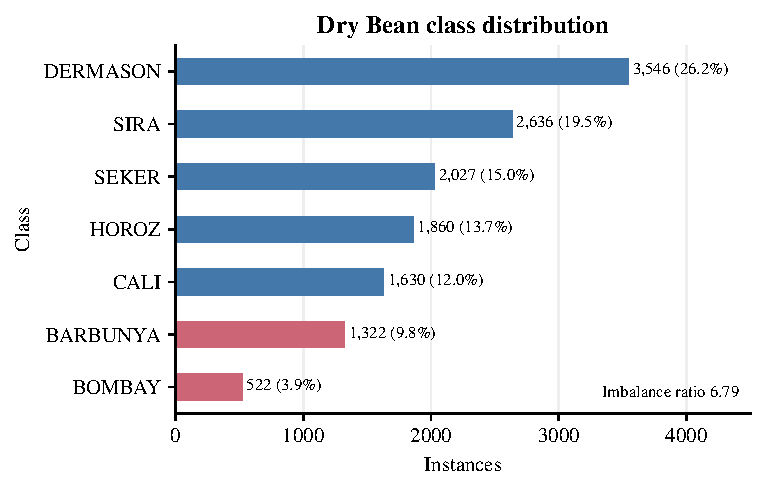
\includegraphics[width=.47\textwidth]{figures/dry_bean/class_distribution.pdf}}\hfill
\subfloat[Steel Plates Faults]{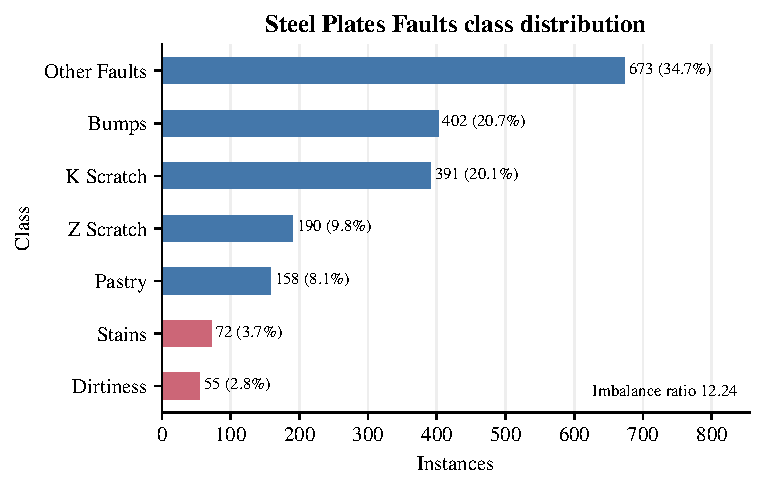
\includegraphics[width=.47\textwidth]{figures/steel_plates/class_distribution.pdf}}
\caption{Class counts after duplicate removal, sorted from least to most frequent. Labels show counts and percentages; the two minority classes are highlighted. Each panel states its largest-to-smallest class ratio. Experimental class order was determined separately within each training fold.}\label{fig:distribution}
\end{figure*}

\subsection{Architecture Selection}
Figure~\ref{fig:architecture} shows the fold-specific validation curves. The selected Dry Bean capacities were 64, 64, 32, 128, and 256 hidden units. Steel Plates selected 256, 64, 256, 512, and 512 units. Steel Plates folds four and five selected the maximum tested capacity of 512 units. Their optima were therefore not bracketed by the search range; 512 is the best tested capacity rather than an established interior optimum.
\begin{figure*}[t]\centering
\subfloat[Dry Bean]{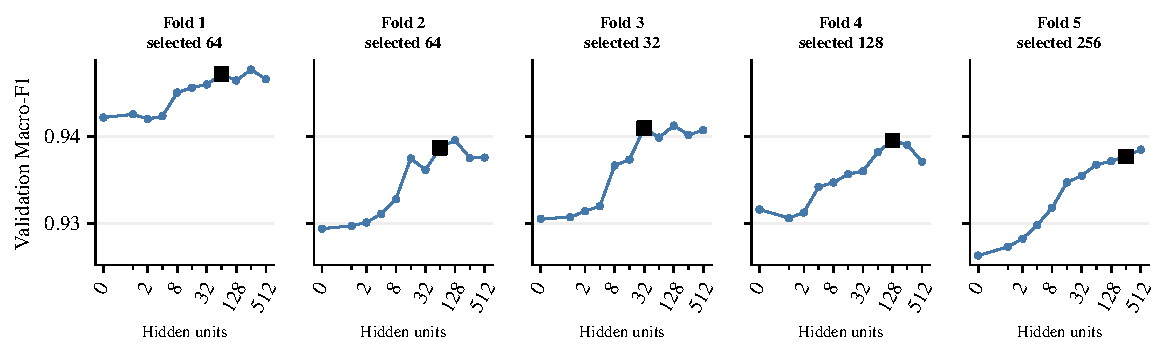
\includegraphics[width=.86\textwidth]{figures/dry_bean/baseline_architecture.pdf}}\\
\subfloat[Steel Plates Faults]{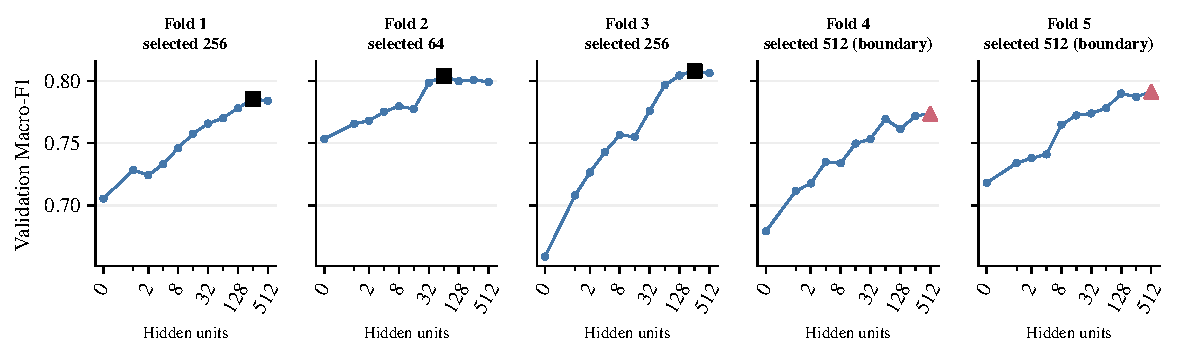
\includegraphics[width=.86\textwidth]{figures/steel_plates/baseline_architecture.pdf}}
\caption{Validation Macro-F1 across tested hidden capacities, shown separately for each outer fold. The larger marker identifies the selected size; triangles identify selections at the maximum tested capacity, which do not establish an interior optimum.}\label{fig:architecture}
\end{figure*}

\subsection{Overall Classification Performance}
\begin{table}[t]
\caption{Overall test performance: Dry Bean}
\label{tab:dry-bean-overall}
\centering
\begin{tabular}{lcc}
\toprule Method & Macro-F1 & Fold std. dev.\\
\midrule
Ordinary baseline & 0.9396 & 0.0069\\
Fixed update-budget control & 0.9405 & 0.0061\\
Dynamic all-classes & 0.9375 & 0.0063\\
Dynamic incremental & 0.9386 & 0.0064\\
Fixed incremental & 0.9412 & 0.0060\\
\bottomrule
\end{tabular}
\end{table}
\begin{table}[t]
\caption{Overall test performance: Steel Plates Faults}
\label{tab:steel-plates-overall}
\centering
\begin{tabular}{lcc}
\toprule Method & Macro-F1 & Fold std. dev.\\
\midrule
Ordinary baseline & 0.7638 & 0.0067\\
Fixed update-budget control & 0.7673 & 0.0070\\
Dynamic all-classes & 0.7312 & 0.0114\\
Dynamic incremental & 0.7348 & 0.0096\\
Fixed incremental & 0.7721 & 0.0075\\
\bottomrule
\end{tabular}
\end{table}

Tables~\ref{tab:dry-bean-overall} and~\ref{tab:steel-plates-overall} report fold-level Macro-F1 means and between-fold standard deviations. Fixed incremental learning had the highest mean on Dry Bean at 0.9412 and on Steel Plates at 0.7721. The ordinary baseline reached 0.9396 and 0.7638, respectively. Dynamic incremental learning reached 0.9386 and 0.7348. Fixed incremental had the highest observed mean Macro-F1 on both datasets. The controlled comparisons below assess the evidence for an effect of class presentation.

\subsection{Controlled Curriculum Effects}
\begin{table*}[t]
\caption{Paired fold-level comparisons: Dry Bean}
\label{tab:dry-bean-statistics}
\centering\small
\resizebox{\textwidth}{!}{\begin{tabular}{llrrrrrr}
\toprule Family & Comparison & Mean diff. & 95\% interval & $d_z$ & Raw $p$ & Holm $p$ & $n$\\
\midrule
Primary & Fixed incremental minus Fixed update-budget control & +0.0007 & [-0.0012, 0.0026] & 0.449 & 0.3725 & 0.3725 & 5\\
Primary & Dynamic incremental minus Dynamic all-classes & +0.0011 & [-0.0002, 0.0024] & 1.069 & 0.0752 & 0.1503 & 5\\
Minority exploratory & Fixed incremental minus Fixed update-budget control & +0.0014 & [-0.0015, 0.0044] & 0.606 & 0.2471 & 0.2471 & 5\\
Minority exploratory & Dynamic incremental minus Dynamic all-classes & +0.0013 & [-0.0005, 0.0031] & 0.878 & 0.1211 & 0.2422 & 5\\
\bottomrule
\end{tabular}}
\end{table*}
\begin{table*}[t]
\caption{Paired fold-level comparisons: Steel Plates Faults}
\label{tab:steel-plates-statistics}
\centering\small
\resizebox{\textwidth}{!}{\begin{tabular}{llrrrrrr}
\toprule Family & Comparison & Mean diff. & 95\% interval & $d_z$ & Raw $p$ & Holm $p$ & $n$\\
\midrule
Primary & Fixed incremental minus Fixed update-budget control & +0.0047 & [-0.0096, 0.0191] & 0.411 & 0.4105 & 0.8210 & 5\\
Primary & Dynamic incremental minus Dynamic all-classes & +0.0037 & [-0.0094, 0.0167] & 0.350 & 0.4781 & 0.8210 & 5\\
Minority exploratory & Fixed incremental minus Fixed update-budget control & +0.0069 & [-0.0194, 0.0331] & 0.324 & 0.5091 & 0.5091 & 5\\
Minority exploratory & Dynamic incremental minus Dynamic all-classes & +0.0151 & [-0.0157, 0.0459] & 0.608 & 0.2456 & 0.4913 & 5\\
\bottomrule
\end{tabular}}
\end{table*}

Tables~\ref{tab:dry-bean-statistics} and~\ref{tab:steel-plates-statistics} report the primary contrasts. Fixed incremental exceeded the matched control by 0.0007 on Dry Bean, with a 95\% interval of $[-0.0012,0.0026]$ and Holm-adjusted $p=0.3725$. The Steel Plates difference was 0.0047, with an interval of $[-0.0096,0.0191]$ and adjusted $p=0.8210$. The point estimates favoured the curriculum, but both intervals contained zero.

Dynamic incremental exceeded dynamic all-classes by 0.0011 on Dry Bean and 0.0037 on Steel Plates. The corresponding intervals were $[-0.0002,0.0024]$ and $[-0.0094,0.0167]$; Holm-adjusted $p$-values were 0.1503 and 0.8210. Figure~\ref{fig:primary-effects} shows all four primary contrasts and their fold-level spread. The dynamic comparison held growth rules constant, yet the observed advantage remained uncertain. All four primary intervals included zero, so the data leave the direction and magnitude of the curriculum effects uncertain.
\begin{figure*}[t]\centering
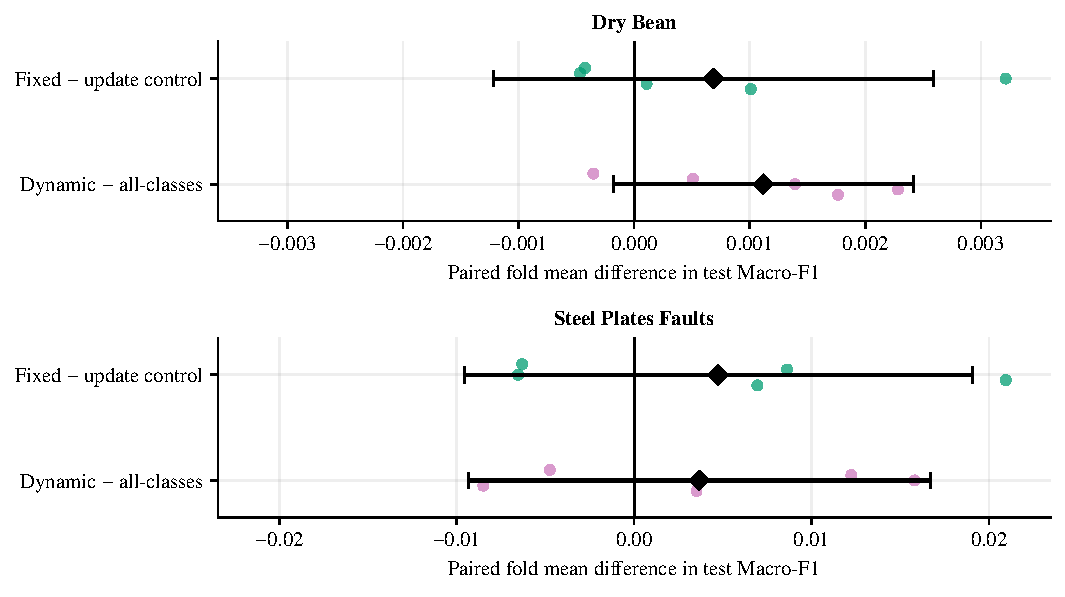
\includegraphics[width=.85\textwidth]{figures/primary_effects.pdf}
\caption{Primary paired test Macro-F1 differences. Small points show the five outer-fold differences after averaging optimisation seeds within each fold. Diamonds show mean paired differences; horizontal bars show unadjusted 95\% confidence intervals. The vertical zero line denotes no observed curriculum effect.}\label{fig:primary-effects}
\end{figure*}

\subsection{Minority and Per-Class Behaviour}
\begin{table}[t]
\caption{Minority performance: Dry Bean}
\label{tab:dry-bean-minority}
\centering
\begin{tabular}{lcc}
\toprule Method & Macro-F1 & Recall\\
\midrule
Ordinary baseline & 0.9657 & 0.9596\\
Fixed update-budget control & 0.9674 & 0.9631\\
Dynamic all-classes & 0.9633 & 0.9561\\
Dynamic incremental & 0.9646 & 0.9585\\
Fixed incremental & 0.9688 & 0.9639\\
\bottomrule
\end{tabular}
\end{table}
\begin{table}[t]
\caption{Minority performance: Steel Plates Faults}
\label{tab:steel-plates-minority}
\centering
\begin{tabular}{lcc}
\toprule Method & Macro-F1 & Recall\\
\midrule
Ordinary baseline & 0.8320 & 0.8226\\
Fixed update-budget control & 0.8438 & 0.8313\\
Dynamic all-classes & 0.7644 & 0.7794\\
Dynamic incremental & 0.7795 & 0.7934\\
Fixed incremental & 0.8506 & 0.8558\\
\bottomrule
\end{tabular}
\end{table}

Tables~\ref{tab:dry-bean-minority} and~\ref{tab:steel-plates-minority} show the same broad ordering as overall Macro-F1. Fixed incremental produced the highest minority Macro-F1 means: 0.9688 on Dry Bean and 0.8506 on Steel Plates. Minority recall was 0.9639 and 0.8558. Relative to the fixed update-budget control, the minority Macro-F1 gains were 0.0014 and 0.0069. Both exploratory 95\% intervals contained zero, so the highest observed means did not establish reliable gains. Dynamic incremental also exceeded dynamic all-classes on the minority metric by 0.0013 and 0.0151, with intervals that included zero. The table retains the exact absolute values; Fig.~\ref{fig:per-class-effects} shows where the paired class-specific differences arose.

The class-specific results were heterogeneous. On Steel Plates, fixed incremental gained 0.0238 for Pastry relative to its matched control, while Other Faults lost 0.0049. Pastry therefore contributed disproportionately to the positive overall point estimate. No class-specific significance claim was made.
\begin{figure*}[t]\centering
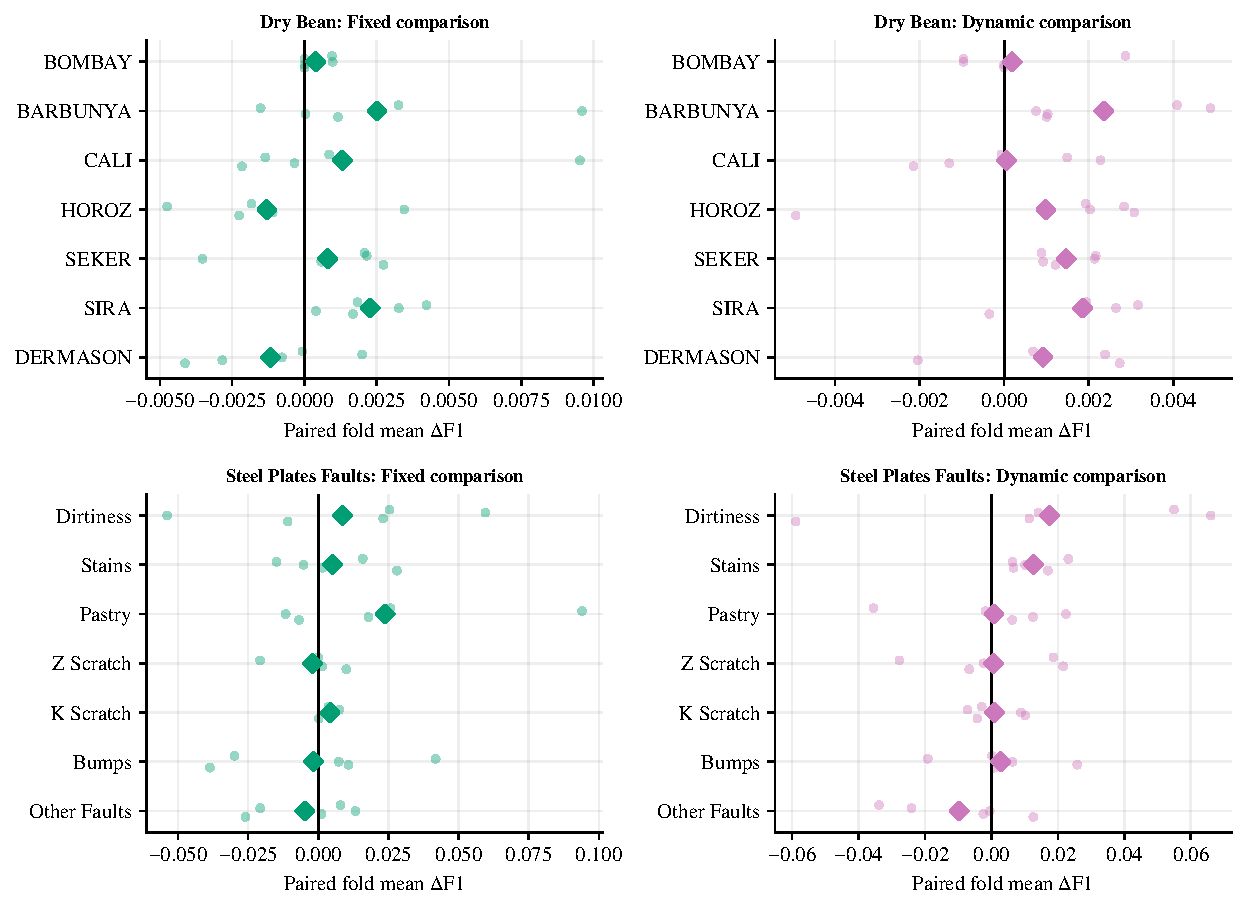
\includegraphics[width=.92\textwidth]{figures/per_class_effects.pdf}
\caption{Descriptive paired class-level test F1 differences for fixed incremental minus its update control and dynamic incremental minus dynamic all-classes. Small points are five outer-fold differences after seed averaging; diamonds are their means. Classes follow full-dataset frequency from rarest at top to most common at bottom; experimental order remained fold-specific. Zero denotes no observed class-level difference.}\label{fig:per-class-effects}
\end{figure*}

\subsection{Dynamic-Capacity Behaviour}
Figure~\ref{fig:progression} shows that validation Macro-F1 fell as more classes entered the curriculum. The five fold trajectories expose variation after averaging seeds within each fold. Each stage changes the classification task, so scores across stages are not like-for-like test comparisons. Figure~\ref{fig:growth} shows the discrete hidden-unit counts from dynamic incremental runs. Dynamic all-classes had only one training stage with all classes available; its mean in Fig.~\ref{fig:growth} is a horizontal reference, separate from the incremental stage axis.

Dynamic all-classes finished with 1.92 hidden units on average in each dataset. Dynamic incremental finished with 4.72 on Dry Bean and 4.96 on Steel Plates. More accepted growth under the curriculum accompanied more probe attempts: dynamic incremental averaged six rejected probes per run, compared with one for dynamic all-classes. The additional probes consumed updates and examples even when growth was rejected.

Figure~\ref{fig:dynamic-capacity-performance} shows each of the 50 dynamic-method runs per dataset by final hidden capacity and test Macro-F1. Capacity was an outcome of the growth procedure, so the observed association is descriptive.
\begin{figure*}[t]\centering
\subfloat[Dry Bean]{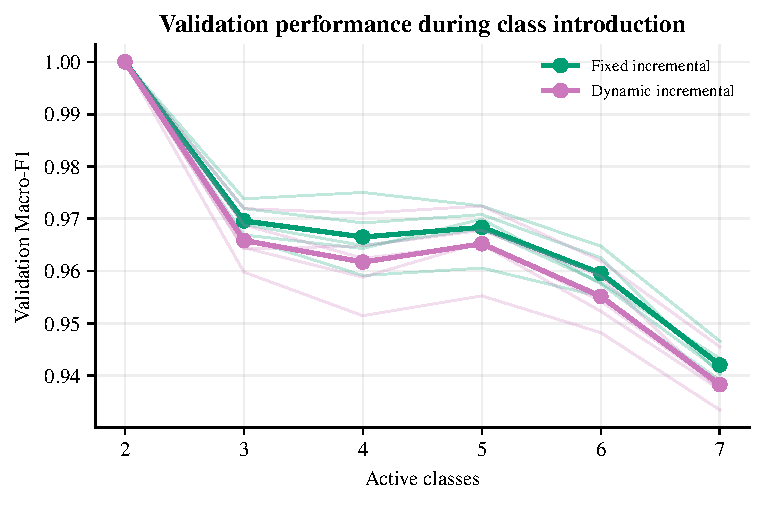
\includegraphics[width=.47\textwidth]{figures/dry_bean/incremental_progression.pdf}}\hfill
\subfloat[Steel Plates Faults]{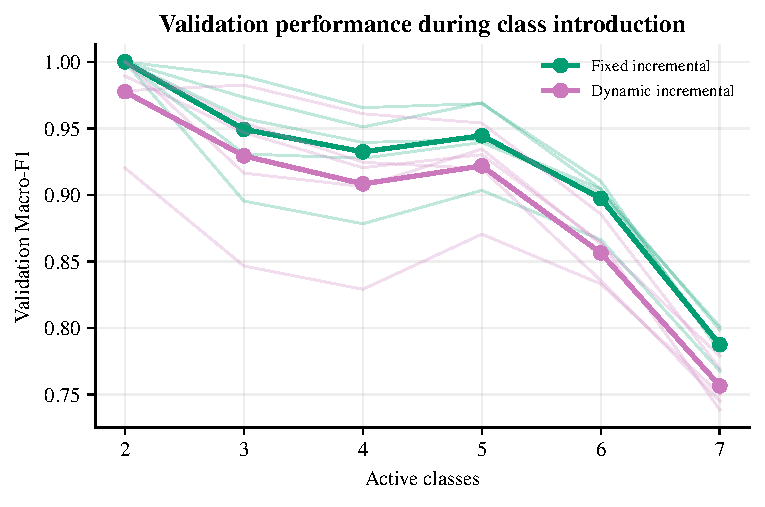
\includegraphics[width=.47\textwidth]{figures/steel_plates/incremental_progression.pdf}}
\caption{Validation Macro-F1 during cumulative class introduction. Thin lines show five outer-fold trajectories after averaging five optimisation seeds within each fold; thick lines show their mean. The task gains a class at each stage, so scores across stages are not like-for-like test comparisons.}\label{fig:progression}
\end{figure*}
\begin{figure*}[t]\centering
\subfloat[Dry Bean]{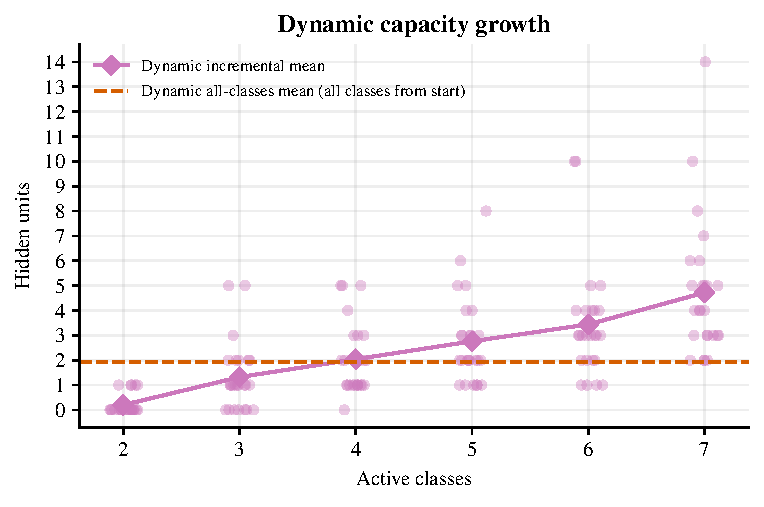
\includegraphics[width=.47\textwidth]{figures/dry_bean/network_growth.pdf}}\hfill
\subfloat[Steel Plates Faults]{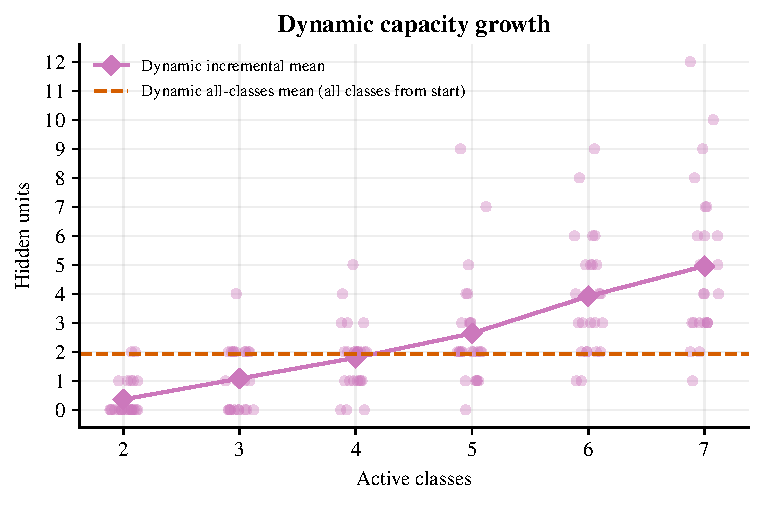
\includegraphics[width=.47\textwidth]{figures/steel_plates/network_growth.pdf}}
\caption{Validation-triggered hidden-capacity growth. Jittered points show all 25 fold and seed runs at each number of active classes; diamonds and their connecting line show stage means. The dashed line shows the dynamic all-classes mean across its 25 single-stage runs, with every class available from the start.}\label{fig:growth}
\end{figure*}
\begin{figure*}[t]\centering
\subfloat[Dry Bean]{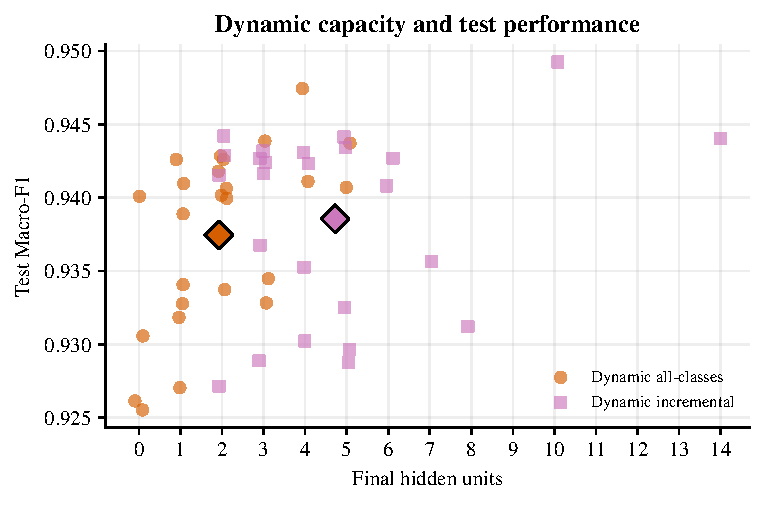
\includegraphics[width=.47\textwidth]{figures/dry_bean/dynamic_capacity_performance.pdf}}\hfill
\subfloat[Steel Plates Faults]{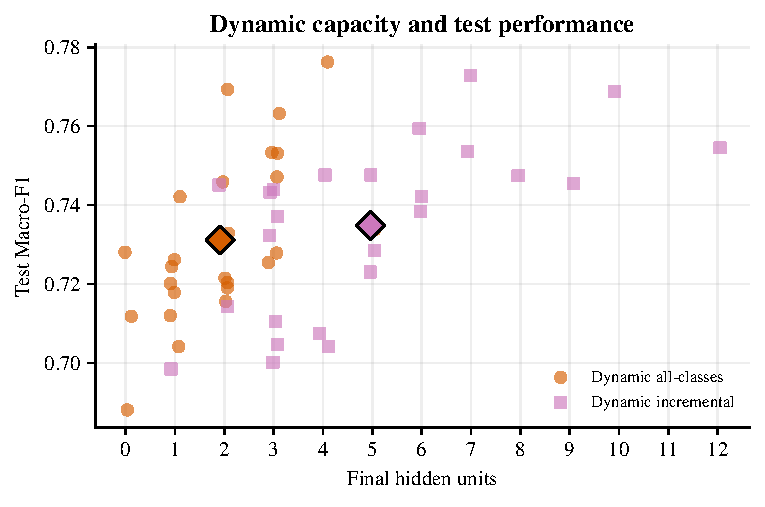
\includegraphics[width=.47\textwidth]{figures/steel_plates/dynamic_capacity_performance.pdf}}
\caption{Observed final hidden units and test Macro-F1 for each dynamic all-classes and dynamic incremental run. Horizontal jitter separates equal integer capacities; large diamonds show method means. Capacity is an outcome of growth, so the association is descriptive.}\label{fig:dynamic-capacity-performance}
\end{figure*}

\subsection{Computational Cost and Cross-Data-Set Comparison}
\begin{table*}[t]
\caption{Training cost: Dry Bean}
\label{tab:dry-bean-efficiency}
\centering\small
\resizebox{\textwidth}{!}{\begin{tabular}{lrrrrrr}
\toprule Method & Mean updates & Mean examples processed & Mean final hidden & Accepted & Rejected & Mean time (s)\\
\midrule
Ordinary baseline & 1766 & 225341 & 108.8 & 0.0 & 0.0 & 1.7\\
Fixed update-budget control & 3844 & 490365 & 108.8 & 0.0 & 0.0 & 3.7\\
Dynamic all-classes & 6798 & 867213 & 1.9 & 1.9 & 1.0 & 1.5\\
Dynamic incremental & 13279 & 1677827 & 4.7 & 4.7 & 6.0 & 3.6\\
Fixed incremental & 3844 & 485332 & 108.8 & 0.0 & 0.0 & 3.8\\
\bottomrule
\end{tabular}}
\end{table*}
\begin{table*}[t]
\caption{Training cost: Steel Plates Faults}
\label{tab:steel-plates-efficiency}
\centering\small
\resizebox{\textwidth}{!}{\begin{tabular}{lrrrrrr}
\toprule Method & Mean updates & Mean examples processed & Mean final hidden & Accepted & Rejected & Mean time (s)\\
\midrule
Ordinary baseline & 264 & 33341 & 320.0 & 0.0 & 0.0 & 0.9\\
Fixed update-budget control & 543 & 68508 & 320.0 & 0.0 & 0.0 & 1.7\\
Dynamic all-classes & 1274 & 160702 & 1.9 & 1.9 & 1.0 & 0.7\\
Dynamic incremental & 2009 & 233601 & 5.0 & 5.0 & 6.0 & 1.9\\
Fixed incremental & 543 & 62887 & 320.0 & 0.0 & 0.0 & 2.1\\
\bottomrule
\end{tabular}}
\end{table*}

Tables~\ref{tab:dry-bean-efficiency} and~\ref{tab:steel-plates-efficiency} and Fig.~\ref{fig:performance-cost} show the capacity--effort trade-off. The fixed incremental networks averaged 108.8 hidden units on Dry Bean and 320.0 on Steel Plates. Dynamic incremental finished with 4.7 and 5.0 units, respectively. Despite the smaller final networks, dynamic incremental required 13,279 updates versus 3,844 for fixed incremental on Dry Bean. Steel Plates required 2,009 versus 543 updates. The dynamic method also processed more examples and attained lower absolute Macro-F1. Mean training time was 3.6 versus 3.8 seconds on Dry Bean and 1.9 versus 2.1 seconds on Steel Plates. These time measurements reflect the measured environment and do not overturn the higher update and example counts.
\begin{figure*}[t]\centering
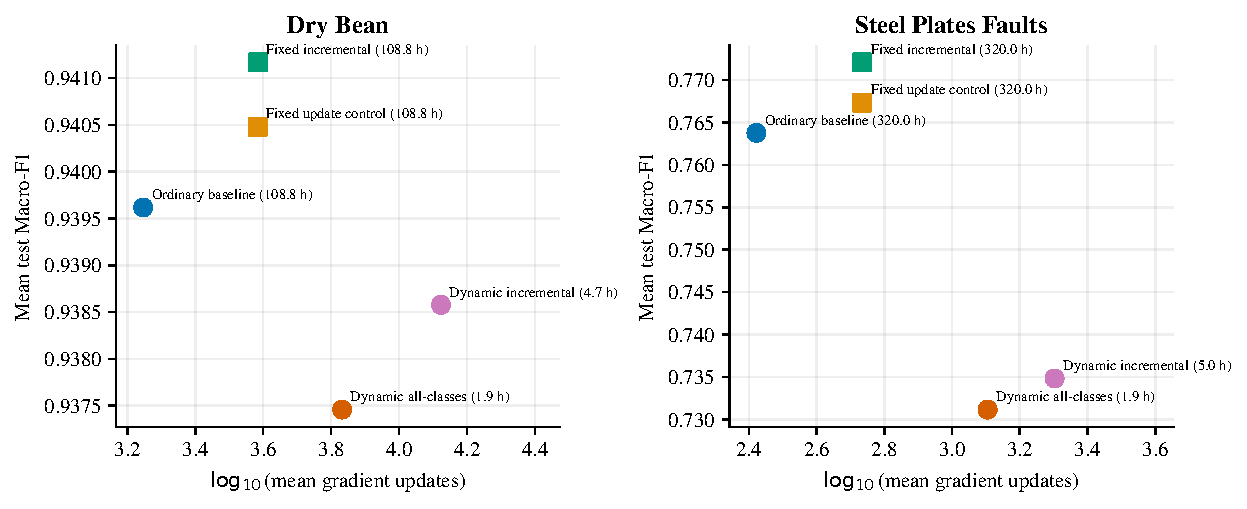
\includegraphics[width=.94\textwidth]{figures/performance_cost.pdf}
\caption{Descriptive performance and optimisation cost for five methods in each dataset. Points show mean test Macro-F1 against mean gradient updates on a logarithmic horizontal scale. Labels give mean final hidden units ($h$); symbol shapes distinguish fixed-capacity methods. The figure compares observed performance, effort, and size without implying a causal effect of any one quantity.}\label{fig:performance-cost}
\end{figure*}

Steel Plates was more imbalanced than Dry Bean, with ratios of 12.24 and 6.79. The ordinary-baseline Macro-F1 was also lower on Steel Plates, at 0.7638 versus 0.9396. The fixed curriculum point estimate relative to its control was larger on Steel Plates, at 0.0047 versus 0.0007; the dynamic estimates were 0.0037 and 0.0011. Wider Steel Plates intervals and the small number of folds prevent attributing the larger observed effects to imbalance or dataset difficulty. The class-specific Pastry gain illustrates why a single aggregate score is insufficient to explain the cross-dataset pattern.

\subsection{Sensitivity and Limitations}
Figure~\ref{fig:sensitivity} shows dynamic incremental validation-only sensitivity to probe duration and minimum accepted gain. Mean Dry Bean validation Macro-F1 ranged from 0.9366 to 0.9404 across the nine settings. Steel Plates ranged from 0.7482 to 0.7567. These spreads, 0.0038 and 0.0085, exceeded the corresponding dynamic curriculum point estimates of 0.0011 and 0.0037 on the test folds. The quantities come from different evaluations and do not measure the same effect, but they show that plausible growth settings materially changed validation performance. A claim that the dynamic conclusion was insensitive to those settings would therefore be premature. The sensitivity grid used validation data and one seed, without test-based selection.
\begin{figure*}[t]\centering
\subfloat[Dry Bean]{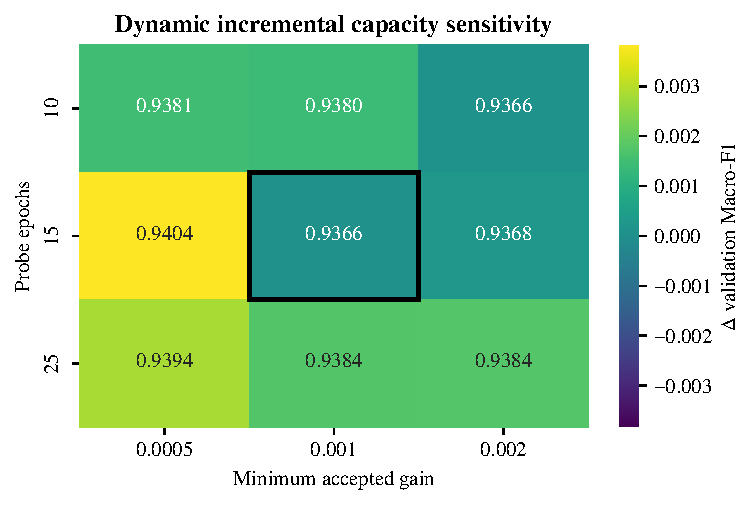
\includegraphics[width=.47\textwidth]{figures/dry_bean/capacity_sensitivity.pdf}}\hfill
\subfloat[Steel Plates Faults]{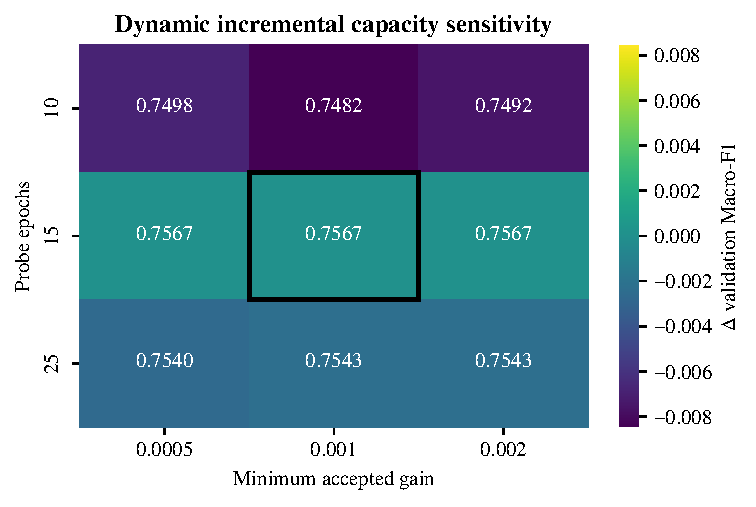
\includegraphics[width=.47\textwidth]{figures/steel_plates/capacity_sensitivity.pdf}}
\caption{Dynamic incremental validation-only capacity sensitivity. Colour shows change in mean validation Macro-F1 relative to the outlined canonical setting (15 probe epochs, minimum gain 0.001); cell text shows absolute mean validation Macro-F1. Each cell averages five inner validation partitions with one fixed optimisation seed. Panels use separate delta colour scales. No test outcomes entered setting selection.}\label{fig:sensitivity}
\end{figure*}

The findings cover two application domains and five test-fold estimates per domain. Outer training partitions overlapped, and the study used one optimiser and a residual classifier architecture. Elapsed times also depend on the execution environment. The intervals and corrected tests therefore support cautious statements about observed fold-level differences, not broad claims of a population-level benefit.

\clearpage
\section{Conclusion}
Fixed incremental learning attained the highest mean overall and minority Macro-F1 on both datasets. Relative to the update-budget control, fixed minority-first presentation produced small positive fold-mean differences of 0.0007 on Dry Bean and 0.0047 on Steel Plates. Dynamic minority-first presentation produced differences of 0.0011 and 0.0037 relative to dynamic all-classes. All four primary 95\% intervals contained zero, and the Holm-adjusted tests did not establish reliable improvements. The results therefore did not demonstrate a dependable benefit from class order alone.

Dynamic growth yielded much smaller final networks than fixed-capacity training. The dynamic methods required more updates and processed more examples, while their absolute Macro-F1 remained lower. The larger observed curriculum effects on Steel Plates coincided with stronger imbalance and lower baseline performance, but the fold-level uncertainty did not support a causal explanation. Two datasets, five overlapping outer training partitions, and sensitivity to growth settings limited generalisation.

\bibliographystyle{IEEEtran}
\setlength{\emergencystretch}{3em}\sloppy
\bibliography{references}
\end{document}
